\section{Experimental Design}

The experimental design of the project was structured into two pipelines: the
Simple Split pipeline and the K-Fold pipeline (Figure \ref{fig:fig2}).

\begin{figure}[H]
	\begin{center}
		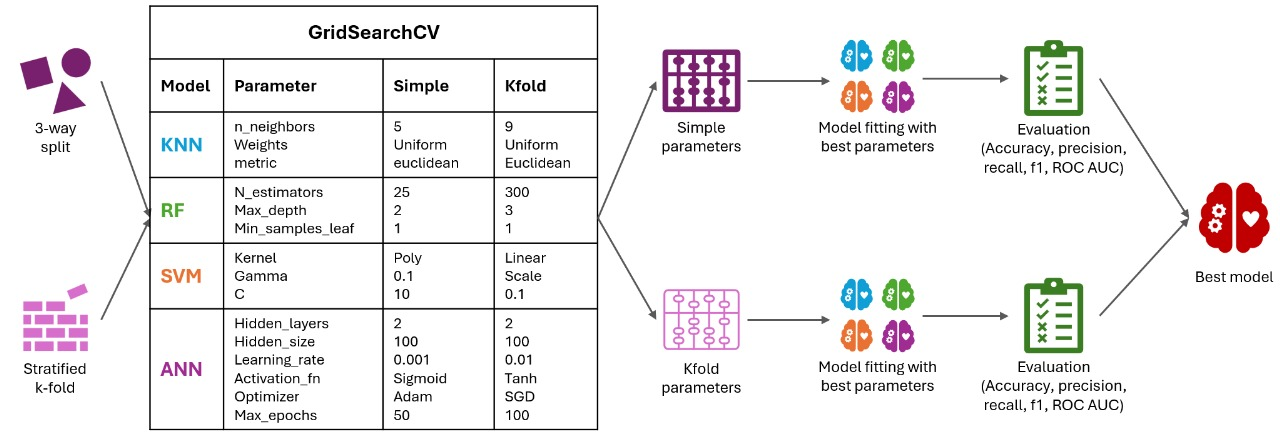
\includegraphics[width=0.99\textwidth]{../images/schemas/workflow_02.jpeg}
	\end{center}
	\caption{Experimental design schema.}
	\label{fig:fig2}
\end{figure}

\subsection{PyRadiomics}

Radiomic features were computed for three cardiac structures: Left Ventricle
(LV), Myocardium (MYO), and Right Ventricle (RV), at two different time points
of the cardiac cycle: End-Systole (ES) and End-Diastole (ED). In
Table \ref{tab:tab2}, we present the various feature classes generated by
PyRadiomics, along with brief descriptions of each.

\begin{table}[H]
	\centering
	\caption{PyRadiomics feature classes and their descriptions.}
	\begin{adjustbox}{width=0.99\textwidth}
		\begin{tabular}{p{3cm}p{15.5cm}}
			\hline
			\textbf{Feature Class} & \textbf{Description}                                                                                                    \\
			\hline
			First-order            & Represents statistical properties of voxel intensities, such as mean, variance, and skewness.                           \\
			Shape                  & Describes the geometric properties of an ROI, including surface area, volume, and sphericity.                           \\
			GLCM                   & Quantifies texture by analyzing the spatial relationships between pixel intensities.                                    \\
			GLRLM                  & Measures the distribution of pixel intensities, focusing on the length of consecutive pixels with the same intensity.   \\
			GLSZM                  & Quantifies the size of homogeneous regions by counting connected voxels with similar intensities.                       \\
			NGTDM                  & Captures local texture variations by measuring differences between a voxel intensity and its neighbors.                 \\
			GLDM                   & Describes the dependency between gray levels in an image, focusing on their spatial arrangement from the central voxel. \\
			\hline
		\end{tabular}
	\end{adjustbox}
	\label{tab:tab2}
\end{table}

\subsection{Feature Selection and Transformation}

The final features selected by the LASSOmodf method were (10): Shape Mesh
Volume LV ED, GLCM Idmn LV ED, GLSZM Large Area High Gray Level Emphasis LV ED,
Shape Elongation LV ES, Shape Mesh Volume RV ES, First Order Kurtosis RV ES,
First Order Skewness RV ES, GLDM Gray Level Non Uniformity RV ES, Shape Minor
Axis Length MYO ES, and NGTDM Coarseness MYO ES. These features were then used
as input for LDA transformation.

\subsection{Model Hyperparameter Tuning}

Hyperparameter optimization was performed using GridSearchCV. In the Annexes
(Figures \ref{fig:figA11} - \ref{fig:figA14}), we illustrate the evolution of
selected hyperparameters across the Simple Split and Stratified K-Fold
pipelines. The Simple Split strategy often results in large discrepancies
between training and validation performance, suggesting overfitting due to
reliance on a single training set. In contrast, the Stratified K-Fold approach
yields more consistent and generally lower scores, indicating improved
generalization and greater stability.

For KNN, the hyperparameters were:

\begin{itemize}
	\item \texttt{n\_neighbors}: Number of neighbors used for classification;
	      higher values yield smoother decision boundaries but may reduce model
	      sensitivity.
	\item \texttt{weights}: Strategy to assign weights to neighbors—either
	      equally (\texttt{uniform}) or inversely proportional to distance
	      (\texttt{distance}).
	\item \texttt{metric}: Distance measure used to compute similarity between
	      data points.
\end{itemize}

For RF, the hyperparameters were:

\begin{itemize}
	\item \texttt{n\_estimators}: Total number of decision trees in the ensemble;
	      more trees generally improve performance but increase computation time.
	\item \texttt{max\_depth}: Maximum allowed depth of each tree; deeper trees
	      can capture complex patterns but risk overfitting.
	\item \texttt{min\_samples\_leaf}: Minimum number of samples required to form
	      a leaf node; higher values constrain model complexity and reduce
	      overfitting.
\end{itemize}

For SVM, the hyperparameters were:

\begin{itemize}
	\item \texttt{kernel}: Function that defines the feature transformation used
	      to separate classes (e.g., linear, RBF, polynomial).
	\item \texttt{gamma}: Defines how far the influence of a single training
	      example reaches; high values create more flexible, complex boundaries.
	\item \texttt{C}: Regularization parameter that balances margin maximization
	      and classification error; lower values favor wider margins.
\end{itemize}

For ANN, the hyperparameters were:

\begin{itemize}
	\item \texttt{hidden\_layers}: Number of hidden layers in the network; deeper
	      networks can model more complex relationships.
	\item \texttt{hidden\_size}: Number of neurons per hidden layer; larger sizes
	      can capture more nuanced features.
	\item \texttt{learning\_rate}: Step size for updating weights during
	      training; controls speed and stability of convergence.
	\item \texttt{activation\_fn}: Non-linear function applied to neurons (e.g.,
	      ReLU, sigmoid); enables learning of complex patterns.
	\item \texttt{optimizer}: Optimization algorithm used for training (e.g.,
	      Adam, SGD); affects convergence rate and stability.
	\item \texttt{max\_epochs}: Maximum number of complete passes through the
	      training data; sets the upper limit for training duration.
\end{itemize}

